% The four readings on the f3-f1 segment: feature 1 alone and features 1 and 3 together
% can produce the same reading (feature i active contributes x_i f_i).
% Compile from figures/ (the fonts resolve relative to the cwd): lualatex naive_cases.tex,
% then pdftoppm -png -r 200 and autocrop to naive_cases.png (see ../reproduce.sh).
\documentclass{article}
\usepackage[a4paper, landscape, margin=1cm]{geometry}
\pagestyle{empty}
\usepackage{fontspec}
\usepackage{xcolor}
\usepackage{amsmath}
\usepackage{tikz}
\setmainfont{Poppins}[
  Path = fonts/Poppins/,
  Extension = .ttf,
  UprightFont = *-Regular,
  BoldFont = *-Bold,
  ItalicFont = *-Italic,
  BoldItalicFont = *-BoldItalic
]
\definecolor{pivotalOrange}{HTML}{F15F22}
\definecolor{pivotalBlue}{HTML}{3A82B5}
\definecolor{pivotalNight}{HTML}{161616}
\definecolor{pivotalTaupe}{HTML}{818089}
\tikzset{
  feat/.style={-stealth, line width=2.4pt, pivotalBlue},
  axis/.style={-stealth, line width=1pt, pivotalTaupe!70},
  drop/.style={dotted, line width=1pt, pivotalTaupe},
  lbl/.style={font=\fontsize{17}{20}\selectfont},
  sm/.style={font=\fontsize{14}{17}\selectfont},
}
\newcommand{\inputsegment}{%
  \draw[axis] (-1.45,0) -- (1.45,0);
  \draw[feat] (0,0) -- (1,0);
  \draw[feat] (0,0) -- (-1,0);
  \node[pivotalBlue, below, lbl] at (1,-0.06)  {$f_1$};
  \node[pivotalBlue, below, lbl] at (-1,-0.06) {$f_3$};
  \fill[pivotalTaupe] (0,0) circle (2pt);}
\begin{document}
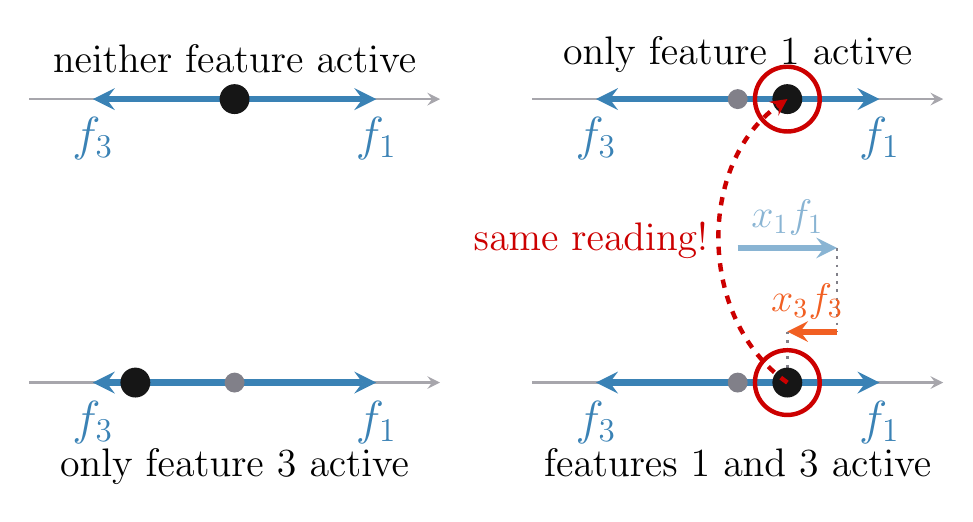
\begin{tikzpicture}[scale=1.8]
  \begin{scope}[shift={(0,0.95)}]
    \inputsegment
    \fill[pivotalNight] (0,0) circle (3pt);
    \node[above, sm] at (0,0.12) {neither feature active};
  \end{scope}
  \begin{scope}[shift={(3.55,0.95)}]
    \inputsegment
    \fill[pivotalNight] (0.35,0) circle (3pt);
    \draw[red!80!black, line width=1.6pt] (0.35,0) circle (6.5pt);
    \node[above, sm] at (0,0.12) {only feature 1 active};
    \coordinate (clashtop) at (0.35,0);
  \end{scope}
  \begin{scope}[shift={(0,-1.05)}]
    \inputsegment
    \fill[pivotalNight] (-0.7,0) circle (3pt);
    \node[below, sm] at (0,-0.4) {only feature 3 active};
  \end{scope}
  \begin{scope}[shift={(3.55,-1.05)}]
    \inputsegment
    \draw[-stealth, line width=2.2pt, pivotalBlue!60] (0,0.95) -- (0.7,0.95)
      node[midway, above, sm] {$x_1 f_1$};
    \draw[drop] (0.7,0.95) -- (0.7,0.36);
    \draw[-stealth, line width=2.2pt, pivotalOrange] (0.7,0.36) -- (0.35,0.36)
      node[pos=0.6, above, sm] {$x_3 f_3$};
    \draw[drop] (0.35,0.36) -- (0.35,0);
    \fill[pivotalNight] (0.35,0) circle (3pt);
    \draw[red!80!black, line width=1.6pt] (0.35,0) circle (6.5pt);
    \node[below, sm] at (0,-0.4) {features 1 and 3 active};
    \coordinate (clashbottom) at (0.35,0);
  \end{scope}
  \draw[red!80!black, dashed, line width=1.6pt, -stealth]
    (clashbottom) to[bend left=55] node[pos=0.5, left, sm] {same reading!} (clashtop);
\end{tikzpicture}
\end{document}
